\documentclass[1p]{elsarticle_modified}
%\bibliographystyle{elsarticle-num}

%\usepackage[colorlinks]{hyperref}
%\usepackage{abbrmath_seonhwa} %\Abb, \Ascr, \Acal ,\Abf, \Afrak
\usepackage{amsfonts}
\usepackage{amssymb}
\usepackage{amsmath}
\usepackage{amsthm}
\usepackage{scalefnt}
\usepackage{amsbsy}
\usepackage{kotex}
\usepackage{caption}
\usepackage{subfig}
\usepackage{color}
\usepackage{graphicx}
\usepackage{xcolor} %% white, black, red, green, blue, cyan, magenta, yellow
\usepackage{float}
\usepackage{setspace}
\usepackage{hyperref}

\usepackage{tikz}
\usetikzlibrary{arrows}

\usepackage{multirow}
\usepackage{array} % fixed length table
\usepackage{hhline}

%%%%%%%%%%%%%%%%%%%%%
\makeatletter
\renewcommand*\env@matrix[1][\arraystretch]{%
	\edef\arraystretch{#1}%
	\hskip -\arraycolsep
	\let\@ifnextchar\new@ifnextchar
	\array{*\c@MaxMatrixCols c}}
\makeatother %https://tex.stackexchange.com/questions/14071/how-can-i-increase-the-line-spacing-in-a-matrix
%%%%%%%%%%%%%%%

\usepackage[normalem]{ulem}

\newcommand{\msout}[1]{\ifmmode\text{\sout{\ensuremath{#1}}}\else\sout{#1}\fi}
%SOURCE: \msout is \stkout macro in https://tex.stackexchange.com/questions/20609/strikeout-in-math-mode

\newcommand{\cancel}[1]{
	\ifmmode
	{\color{red}\msout{#1}}
	\else
	{\color{red}\sout{#1}}
	\fi
}

\newcommand{\add}[1]{
	{\color{blue}\uwave{#1}}
}

\newcommand{\replace}[2]{
	\ifmmode
	{\color{red}\msout{#1}}{\color{blue}\uwave{#2}}
	\else
	{\color{red}\sout{#1}}{\color{blue}\uwave{#2}}
	\fi
}

\newcommand{\Sol}{\mathcal{S}} %segment
\newcommand{\D}{D} %diagram
\newcommand{\A}{\mathcal{A}} %arc


%%%%%%%%%%%%%%%%%%%%%%%%%%%%%5 test

\def\sl{\operatorname{\textup{SL}}(2,\Cbb)}
\def\psl{\operatorname{\textup{PSL}}(2,\Cbb)}
\def\quan{\mkern 1mu \triangleright \mkern 1mu}

\theoremstyle{definition}
\newtheorem{thm}{Theorem}[section]
\newtheorem{prop}[thm]{Proposition}
\newtheorem{lem}[thm]{Lemma}
\newtheorem{ques}[thm]{Question}
\newtheorem{cor}[thm]{Corollary}
\newtheorem{defn}[thm]{Definition}
\newtheorem{exam}[thm]{Example}
\newtheorem{rmk}[thm]{Remark}
\newtheorem{alg}[thm]{Algorithm}

\newcommand{\I}{\sqrt{-1}}
\begin{document}

%\begin{frontmatter}
%
%\title{Boundary parabolic representations of knots up to 8 crossings}
%
%%% Group authors per affiliation:
%\author{Yunhi Cho} 
%\address{Department of Mathematics, University of Seoul, Seoul, Korea}
%\ead{yhcho@uos.ac.kr}
%
%
%\author{Seonhwa Kim} %\fnref{s_kim}}
%\address{Center for Geometry and Physics, Institute for Basic Science, Pohang, 37673, Korea}
%\ead{ryeona17@ibs.re.kr}
%
%\author{Hyuk Kim}
%\address{Department of Mathematical Sciences, Seoul National University, Seoul 08826, Korea}
%\ead{hyukkim@snu.ac.kr}
%
%\author{Seokbeom Yoon}
%\address{Department of Mathematical Sciences, Seoul National University, Seoul, 08826,  Korea}
%\ead{sbyoon15@snu.ac.kr}
%
%\begin{abstract}
%We find all boundary parabolic representation of knots up to 8 crossings.
%
%\end{abstract}
%\begin{keyword}
%    \MSC[2010] 57M25 
%\end{keyword}
%
%\end{frontmatter}

%\linenumbers
%\tableofcontents
%
\newcommand\colored[1]{\textcolor{white}{\rule[-0.35ex]{0.8em}{1.4ex}}\kern-0.8em\color{red} #1}%
%\newcommand\colored[1]{\textcolor{white}{ #1}\kern-2.17ex	\textcolor{white}{ #1}\kern-1.81ex	\textcolor{white}{ #1}\kern-2.15ex\color{red}#1	}

{\Large $\underline{12a_{1126}~(K12a_{1126})}$}

\setlength{\tabcolsep}{10pt}
\renewcommand{\arraystretch}{1.6}
\vspace{1cm}\begin{tabular}{m{100pt}>{\centering\arraybackslash}m{274pt}}
\multirow{5}{120pt}{
	\centering
	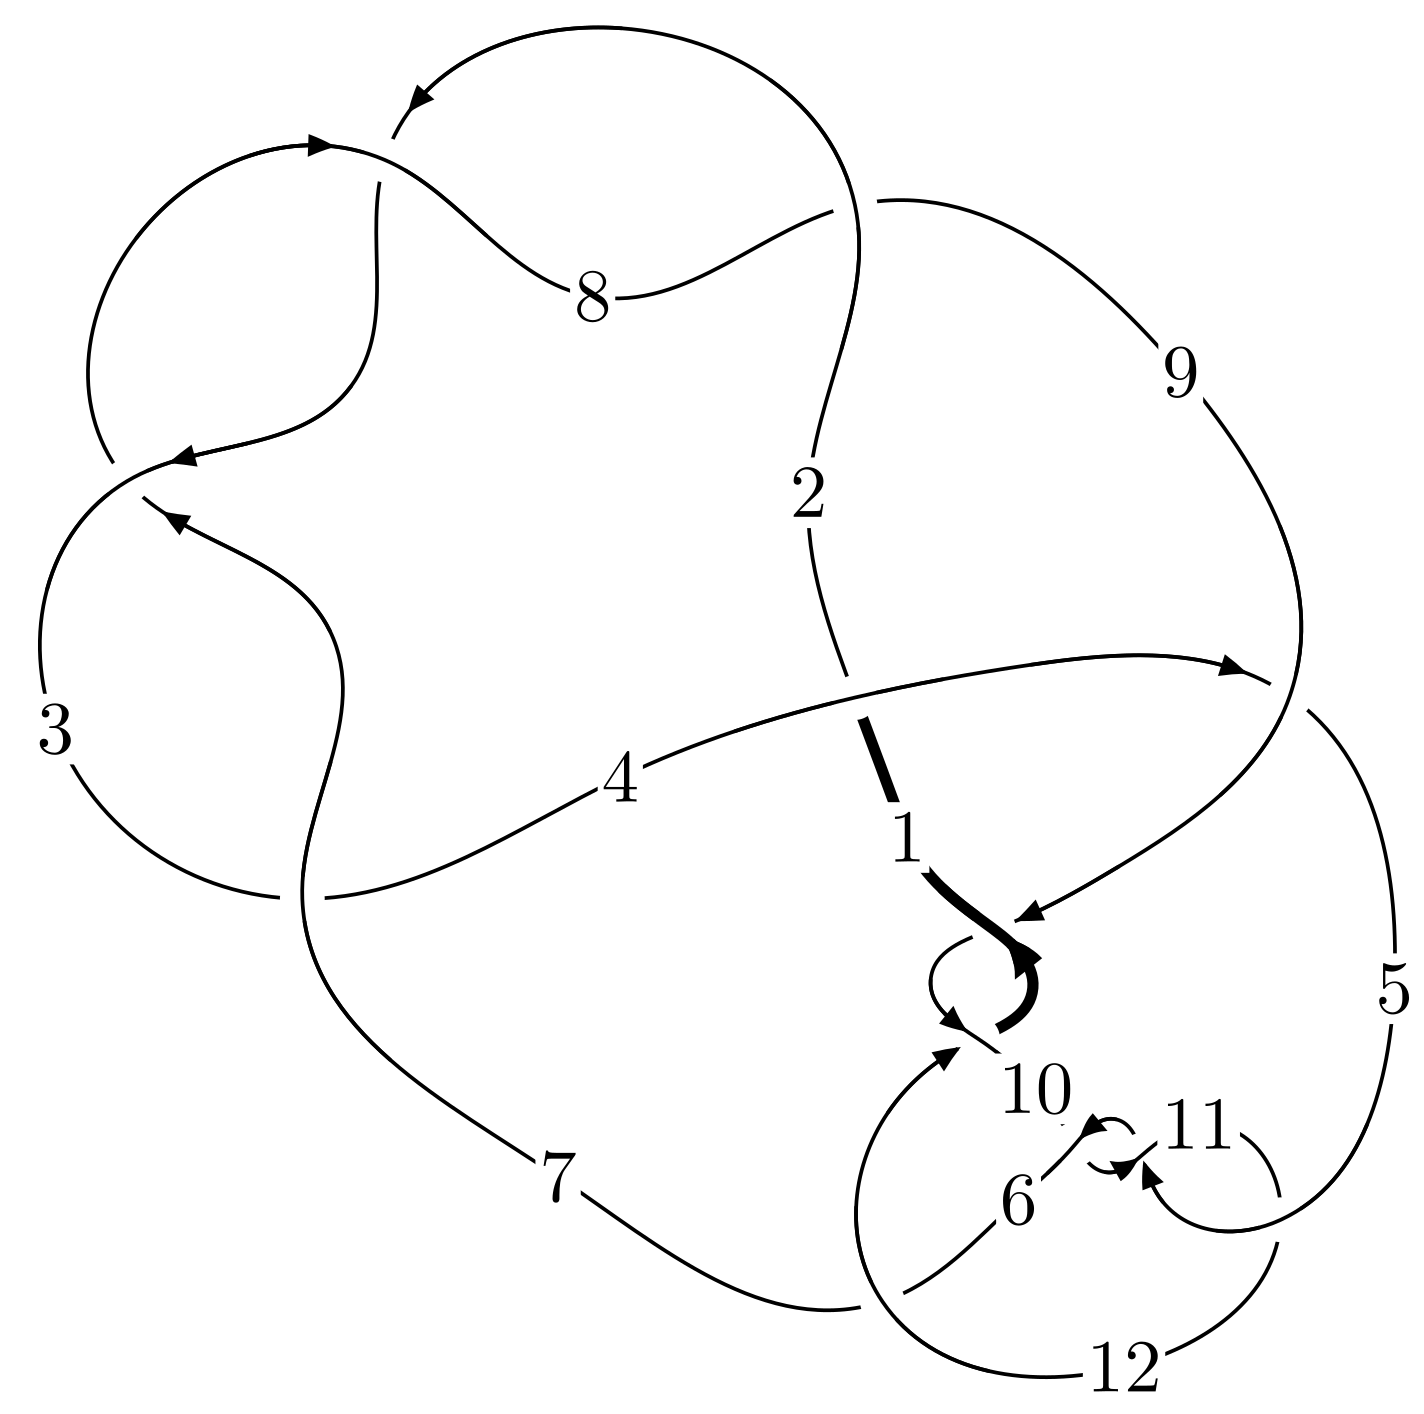
\includegraphics[width=112pt]{../../../GIT/diagram.site/Diagrams/png/1927_12a_1126.png}\\
\ \ \ A knot diagram\footnotemark}&
\allowdisplaybreaks
\textbf{Linearized knot diagam} \\
\cline{2-2}
 &
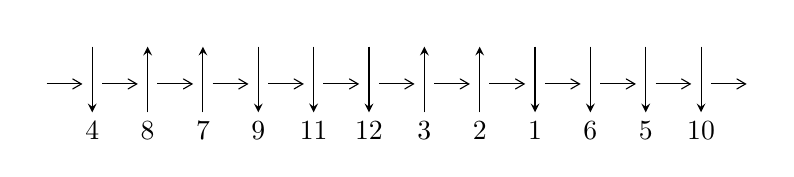
\begin{tikzpicture}[x=20pt, y=17pt]
	% nodes
	\node (C0) at (0, 0) {};
	\node (C1) at (1, 0) {};
	\node (C1U) at (1, +1) {};
	\node (C1D) at (1, -1) {4};

	\node (C2) at (2, 0) {};
	\node (C2U) at (2, +1) {};
	\node (C2D) at (2, -1) {8};

	\node (C3) at (3, 0) {};
	\node (C3U) at (3, +1) {};
	\node (C3D) at (3, -1) {7};

	\node (C4) at (4, 0) {};
	\node (C4U) at (4, +1) {};
	\node (C4D) at (4, -1) {9};

	\node (C5) at (5, 0) {};
	\node (C5U) at (5, +1) {};
	\node (C5D) at (5, -1) {11};

	\node (C6) at (6, 0) {};
	\node (C6U) at (6, +1) {};
	\node (C6D) at (6, -1) {12};

	\node (C7) at (7, 0) {};
	\node (C7U) at (7, +1) {};
	\node (C7D) at (7, -1) {3};

	\node (C8) at (8, 0) {};
	\node (C8U) at (8, +1) {};
	\node (C8D) at (8, -1) {2};

	\node (C9) at (9, 0) {};
	\node (C9U) at (9, +1) {};
	\node (C9D) at (9, -1) {1};

	\node (C10) at (10, 0) {};
	\node (C10U) at (10, +1) {};
	\node (C10D) at (10, -1) {6};

	\node (C11) at (11, 0) {};
	\node (C11U) at (11, +1) {};
	\node (C11D) at (11, -1) {5};

	\node (C12) at (12, 0) {};
	\node (C12U) at (12, +1) {};
	\node (C12D) at (12, -1) {10};
	\node (C13) at (13, 0) {};

	% arrows
	\draw[->,>={angle 60}]
	(C0) edge (C1) (C1) edge (C2) (C2) edge (C3) (C3) edge (C4) (C4) edge (C5) (C5) edge (C6) (C6) edge (C7) (C7) edge (C8) (C8) edge (C9) (C9) edge (C10) (C10) edge (C11) (C11) edge (C12) (C12) edge (C13) ;	\draw[->,>=stealth]
	(C1U) edge (C1D) (C2D) edge (C2U) (C3D) edge (C3U) (C4U) edge (C4D) (C5U) edge (C5D) (C6U) edge (C6D) (C7D) edge (C7U) (C8D) edge (C8U) (C9U) edge (C9D) (C10U) edge (C10D) (C11U) edge (C11D) (C12U) edge (C12D) ;
	\end{tikzpicture} \\
\hhline{~~} \\& 
\textbf{Solving Sequence} \\ \cline{2-2} 
 &
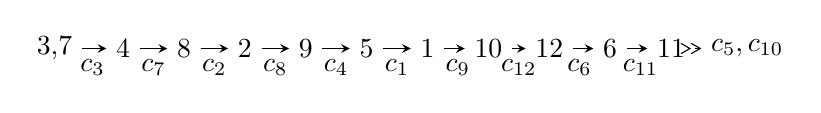
\begin{tikzpicture}[x=22pt, y=7pt]
	% node
	\node (A0) at (-1/8, 0) {3,7};
	\node (A1) at (1, 0) {4};
	\node (A2) at (2, 0) {8};
	\node (A3) at (3, 0) {2};
	\node (A4) at (4, 0) {9};
	\node (A5) at (5, 0) {5};
	\node (A6) at (6, 0) {1};
	\node (A7) at (7, 0) {10};
	\node (A8) at (8, 0) {12};
	\node (A9) at (9, 0) {6};
	\node (A10) at (10, 0) {11};
	\node (C1) at (1/2, -1) {$c_{3}$};
	\node (C2) at (3/2, -1) {$c_{7}$};
	\node (C3) at (5/2, -1) {$c_{2}$};
	\node (C4) at (7/2, -1) {$c_{8}$};
	\node (C5) at (9/2, -1) {$c_{4}$};
	\node (C6) at (11/2, -1) {$c_{1}$};
	\node (C7) at (13/2, -1) {$c_{9}$};
	\node (C8) at (15/2, -1) {$c_{12}$};
	\node (C9) at (17/2, -1) {$c_{6}$};
	\node (C10) at (19/2, -1) {$c_{11}$};
	\node (A11) at (45/4, 0) {$c_{5},c_{10}$};

	% edge
	\draw[->,>=stealth]	
	(A0) edge (A1) (A1) edge (A2) (A2) edge (A3) (A3) edge (A4) (A4) edge (A5) (A5) edge (A6) (A6) edge (A7) (A7) edge (A8) (A8) edge (A9) (A9) edge (A10) ;
	\draw[->>,>={angle 60}]	
	(A10) edge (A11);
\end{tikzpicture} \\ 

\end{tabular} \\

\footnotetext{
The image of knot diagram is generated by the software ``\textbf{Draw programme}" developed by Andrew Bartholomew(\url{http://www.layer8.co.uk/maths/draw/index.htm\#Running-draw}), where we modified some parts for our purpose(\url{https://github.com/CATsTAILs/LinksPainter}).
}\phantom \\ \newline 
\centering \textbf{Ideals for irreducible components\footnotemark of $X_{\text{par}}$} 
 
\begin{align*}
I^u_{1}&=\langle 
u^{59}- u^{58}+\cdots-2 u+1\rangle \\
\\
\end{align*}
\raggedright * 1 irreducible components of $\dim_{\mathbb{C}}=0$, with total 59 representations.\\
\footnotetext{All coefficients of polynomials are rational numbers. But the coefficients are sometimes approximated in decimal forms when there is not enough margin.}
\newpage
\renewcommand{\arraystretch}{1}
\centering \section*{I. $I^u_{1}= \langle u^{59}- u^{58}+\cdots-2 u+1 \rangle$}
\flushleft \textbf{(i) Arc colorings}\\
\begin{tabular}{m{7pt} m{180pt} m{7pt} m{180pt} }
\flushright $a_{3}=$&$\begin{pmatrix}1\\0\end{pmatrix}$ \\
\flushright $a_{7}=$&$\begin{pmatrix}0\\u\end{pmatrix}$ \\
\flushright $a_{4}=$&$\begin{pmatrix}1\\- u^2\end{pmatrix}$ \\
\flushright $a_{8}=$&$\begin{pmatrix}u\\u\end{pmatrix}$ \\
\flushright $a_{2}=$&$\begin{pmatrix}u^2+1\\u^2\end{pmatrix}$ \\
\flushright $a_{9}=$&$\begin{pmatrix}u^3+2 u\\u^3+u\end{pmatrix}$ \\
\flushright $a_{5}=$&$\begin{pmatrix}u^8+5 u^6+7 u^4+2 u^2+1\\u^8+4 u^6+4 u^4\end{pmatrix}$ \\
\flushright $a_{1}=$&$\begin{pmatrix}u^4+3 u^2+1\\- u^6-2 u^4+u^2\end{pmatrix}$ \\
\flushright $a_{10}=$&$\begin{pmatrix}- u^{13}-8 u^{11}-23 u^9-28 u^7-14 u^5-4 u^3+u\\u^{15}+7 u^{13}+16 u^{11}+11 u^9-2 u^7+u\end{pmatrix}$ \\
\flushright $a_{12}=$&$\begin{pmatrix}u^{22}+13 u^{20}+\cdots+2 u^2+1\\- u^{24}-12 u^{22}+\cdots-8 u^6-4 u^4\end{pmatrix}$ \\
\flushright $a_{6}=$&$\begin{pmatrix}u^{45}+26 u^{43}+\cdots+4 u^3+u\\- u^{47}-25 u^{45}+\cdots-4 u^5+u\end{pmatrix}$ \\
\flushright $a_{11}=$&$\begin{pmatrix}- u^{40}-23 u^{38}+\cdots+2 u^2+1\\- u^{40}-22 u^{38}+\cdots-8 u^6-4 u^4\end{pmatrix}$\\&\end{tabular}
\flushleft \textbf{(ii) Obstruction class $= -1$}\\~\\
\flushleft \textbf{(iii) Cusp Shapes $= -4 u^{58}+4 u^{57}+\cdots-12 u+2$}\\~\\
\newpage\renewcommand{\arraystretch}{1}
\flushleft \textbf{(iv) u-Polynomials at the component}\newline \\
\begin{tabular}{m{50pt}|m{274pt}}
Crossings & \hspace{64pt}u-Polynomials at each crossing \\
\hline $$\begin{aligned}c_{1}\end{aligned}$$&$\begin{aligned}
&u^{59}-15 u^{58}+\cdots+16 u-1
\end{aligned}$\\
\hline $$\begin{aligned}c_{2},c_{3},c_{7}\\c_{8}\end{aligned}$$&$\begin{aligned}
&u^{59}- u^{58}+\cdots-2 u+1
\end{aligned}$\\
\hline $$\begin{aligned}c_{4}\end{aligned}$$&$\begin{aligned}
&u^{59}- u^{58}+\cdots-60 u+29
\end{aligned}$\\
\hline $$\begin{aligned}c_{5},c_{10},c_{11}\end{aligned}$$&$\begin{aligned}
&u^{59}- u^{58}+\cdots+u^2+1
\end{aligned}$\\
\hline $$\begin{aligned}c_{6}\end{aligned}$$&$\begin{aligned}
&u^{59}+u^{58}+\cdots-32 u+185
\end{aligned}$\\
\hline $$\begin{aligned}c_{9},c_{12}\end{aligned}$$&$\begin{aligned}
&u^{59}-9 u^{58}+\cdots-312 u+17
\end{aligned}$\\
\hline
\end{tabular}\\~\\
\newpage\renewcommand{\arraystretch}{1}
\flushleft \textbf{(v) Riley Polynomials at the component}\newline \\
\begin{tabular}{m{50pt}|m{274pt}}
Crossings & \hspace{64pt}Riley Polynomials at each crossing \\
\hline $$\begin{aligned}c_{1}\end{aligned}$$&$\begin{aligned}
&y^{59}- y^{58}+\cdots-66 y-1
\end{aligned}$\\
\hline $$\begin{aligned}c_{2},c_{3},c_{7}\\c_{8}\end{aligned}$$&$\begin{aligned}
&y^{59}+67 y^{58}+\cdots-2 y-1
\end{aligned}$\\
\hline $$\begin{aligned}c_{4}\end{aligned}$$&$\begin{aligned}
&y^{59}-9 y^{58}+\cdots+8762 y-841
\end{aligned}$\\
\hline $$\begin{aligned}c_{5},c_{10},c_{11}\end{aligned}$$&$\begin{aligned}
&y^{59}+55 y^{58}+\cdots-2 y-1
\end{aligned}$\\
\hline $$\begin{aligned}c_{6}\end{aligned}$$&$\begin{aligned}
&y^{59}+19 y^{58}+\cdots-707526 y-34225
\end{aligned}$\\
\hline $$\begin{aligned}c_{9},c_{12}\end{aligned}$$&$\begin{aligned}
&y^{59}+47 y^{58}+\cdots-338 y-289
\end{aligned}$\\
\hline
\end{tabular}\\~\\
\newpage\flushleft \textbf{(vi) Complex Volumes and Cusp Shapes}
$$\begin{array}{c|c|c}  
\text{Solutions to }I^u_{1}& \I (\text{vol} + \sqrt{-1}CS) & \text{Cusp shape}\\
 \hline 
\begin{aligned}
u &= \phantom{-}0.087204 + 0.851478 I\end{aligned}
 & \phantom{-}5.17243 - 4.73662 I & -4.00000 + 2.76071 I \\ \hline\begin{aligned}
u &= \phantom{-}0.087204 - 0.851478 I\end{aligned}
 & \phantom{-}5.17243 + 4.73662 I & -4.00000 - 2.76071 I \\ \hline\begin{aligned}
u &= \phantom{-}0.522294 + 0.671217 I\end{aligned}
 & \phantom{-}7.75645 + 10.78740 I & -0.55320 - 8.84457 I \\ \hline\begin{aligned}
u &= \phantom{-}0.522294 - 0.671217 I\end{aligned}
 & \phantom{-}7.75645 - 10.78740 I & -0.55320 + 8.84457 I \\ \hline\begin{aligned}
u &= -0.509216 + 0.664867 I\end{aligned}
 & \phantom{-}1.80756 - 7.41238 I & -4.27230 + 9.26004 I \\ \hline\begin{aligned}
u &= -0.509216 - 0.664867 I\end{aligned}
 & \phantom{-}1.80756 + 7.41238 I & -4.27230 - 9.26004 I \\ \hline\begin{aligned}
u &= -0.522330 + 0.627830 I\end{aligned}
 & \phantom{-}8.64971 - 0.66019 I & \phantom{-}1.00927 + 3.06229 I \\ \hline\begin{aligned}
u &= -0.522330 - 0.627830 I\end{aligned}
 & \phantom{-}8.64971 + 0.66019 I & \phantom{-}1.00927 - 3.06229 I \\ \hline\begin{aligned}
u &= \phantom{-}0.502304 + 0.642574 I\end{aligned}
 & \phantom{-}2.30495 + 3.34683 I & -2.71079 - 3.11364 I \\ \hline\begin{aligned}
u &= \phantom{-}0.502304 - 0.642574 I\end{aligned}
 & \phantom{-}2.30495 - 3.34683 I & -2.71079 + 3.11364 I \\ \hline\begin{aligned}
u &= \phantom{-}0.423758 + 0.695721 I\end{aligned}
 & \phantom{-}1.01542 + 5.69298 I & -5.32566 - 8.42870 I \\ \hline\begin{aligned}
u &= \phantom{-}0.423758 - 0.695721 I\end{aligned}
 & \phantom{-}1.01542 - 5.69298 I & -5.32566 + 8.42870 I \\ \hline\begin{aligned}
u &= -0.373673 + 0.691083 I\end{aligned}
 & -3.05801 - 2.71446 I & -12.01209 + 6.09741 I \\ \hline\begin{aligned}
u &= -0.373673 - 0.691083 I\end{aligned}
 & -3.05801 + 2.71446 I & -12.01209 - 6.09741 I \\ \hline\begin{aligned}
u &= \phantom{-}0.301840 + 0.720122 I\end{aligned}
 & \phantom{-}0.268239 - 0.062723 I & -7.61119 - 1.27500 I \\ \hline\begin{aligned}
u &= \phantom{-}0.301840 - 0.720122 I\end{aligned}
 & \phantom{-}0.268239 + 0.062723 I & -7.61119 + 1.27500 I \\ \hline\begin{aligned}
u &= -0.085060 + 0.774106 I\end{aligned}
 & -0.61920 + 1.71941 I & -8.31003 - 3.37529 I \\ \hline\begin{aligned}
u &= -0.085060 - 0.774106 I\end{aligned}
 & -0.61920 - 1.71941 I & -8.31003 + 3.37529 I \\ \hline\begin{aligned}
u &= -0.573822 + 0.292341 I\end{aligned}
 & \phantom{-}9.62917 - 3.10105 I & \phantom{-}3.62624 + 3.32555 I \\ \hline\begin{aligned}
u &= -0.573822 - 0.292341 I\end{aligned}
 & \phantom{-}9.62917 + 3.10105 I & \phantom{-}3.62624 - 3.32555 I \\ \hline\begin{aligned}
u &= -0.445524 + 0.459511 I\end{aligned}
 & \phantom{-}5.05128 - 1.59378 I & \phantom{-}2.60026 + 4.57588 I \\ \hline\begin{aligned}
u &= -0.445524 - 0.459511 I\end{aligned}
 & \phantom{-}5.05128 + 1.59378 I & \phantom{-}2.60026 - 4.57588 I \\ \hline\begin{aligned}
u &= \phantom{-}0.592961 + 0.236270 I\end{aligned}
 & \phantom{-}9.02899 - 6.97871 I & \phantom{-}2.70616 + 3.27231 I \\ \hline\begin{aligned}
u &= \phantom{-}0.592961 - 0.236270 I\end{aligned}
 & \phantom{-}9.02899 + 6.97871 I & \phantom{-}2.70616 - 3.27231 I \\ \hline\begin{aligned}
u &= -0.570616 + 0.237617 I\end{aligned}
 & \phantom{-}3.05307 + 3.70586 I & -0.77253 - 3.59782 I \\ \hline\begin{aligned}
u &= -0.570616 - 0.237617 I\end{aligned}
 & \phantom{-}3.05307 - 3.70586 I & -0.77253 + 3.59782 I \\ \hline\begin{aligned}
u &= \phantom{-}0.552309 + 0.268389 I\end{aligned}
 & \phantom{-}3.39541 + 0.29109 I & \phantom{-}0.41142 - 3.33717 I \\ \hline\begin{aligned}
u &= \phantom{-}0.552309 - 0.268389 I\end{aligned}
 & \phantom{-}3.39541 - 0.29109 I & \phantom{-}0.41142 + 3.33717 I \\ \hline\begin{aligned}
u &= -0.029521 + 1.409530 I\end{aligned}
 & \phantom{-}4.52945 - 5.12440 I & \phantom{-0.000000 } 0 \\ \hline\begin{aligned}
u &= -0.029521 - 1.409530 I\end{aligned}
 & \phantom{-}4.52945 + 5.12440 I & \phantom{-0.000000 } 0\\
 \hline 
 \end{array}$$\newpage$$\begin{array}{c|c|c}  
\text{Solutions to }I^u_{1}& \I (\text{vol} + \sqrt{-1}CS) & \text{Cusp shape}\\
 \hline 
\begin{aligned}
u &= \phantom{-}0.263506 + 0.518367 I\end{aligned}
 & -0.175692 + 1.026690 I & -3.26382 - 6.43248 I \\ \hline\begin{aligned}
u &= \phantom{-}0.263506 - 0.518367 I\end{aligned}
 & -0.175692 - 1.026690 I & -3.26382 + 6.43248 I \\ \hline\begin{aligned}
u &= \phantom{-}0.01406 + 1.42792 I\end{aligned}
 & -1.64302 + 2.04334 I & \phantom{-0.000000 } 0 \\ \hline\begin{aligned}
u &= \phantom{-}0.01406 - 1.42792 I\end{aligned}
 & -1.64302 - 2.04334 I & \phantom{-0.000000 } 0 \\ \hline\begin{aligned}
u &= \phantom{-}0.490035 + 0.102215 I\end{aligned}
 & \phantom{-}2.69779 - 2.53971 I & -0.68814 + 3.21089 I \\ \hline\begin{aligned}
u &= \phantom{-}0.490035 - 0.102215 I\end{aligned}
 & \phantom{-}2.69779 + 2.53971 I & -0.68814 - 3.21089 I \\ \hline\begin{aligned}
u &= -0.08759 + 1.53351 I\end{aligned}
 & -1.60105 - 3.31687 I & \phantom{-0.000000 } 0 \\ \hline\begin{aligned}
u &= -0.08759 - 1.53351 I\end{aligned}
 & -1.60105 + 3.31687 I & \phantom{-0.000000 } 0 \\ \hline\begin{aligned}
u &= -0.423131\phantom{ +0.000000I}\end{aligned}
 & -1.20479\phantom{ +0.000000I} & -7.49580\phantom{ +0.000000I} \\ \hline\begin{aligned}
u &= \phantom{-}0.07142 + 1.57608 I\end{aligned}
 & -7.46190 + 2.18967 I & \phantom{-0.000000 } 0 \\ \hline\begin{aligned}
u &= \phantom{-}0.07142 - 1.57608 I\end{aligned}
 & -7.46190 - 2.18967 I & \phantom{-0.000000 } 0 \\ \hline\begin{aligned}
u &= -0.15017 + 1.57667 I\end{aligned}
 & \phantom{-}1.23526 - 3.11687 I & \phantom{-0.000000 } 0 \\ \hline\begin{aligned}
u &= -0.15017 - 1.57667 I\end{aligned}
 & \phantom{-}1.23526 + 3.11687 I & \phantom{-0.000000 } 0 \\ \hline\begin{aligned}
u &= \phantom{-}0.14422 + 1.58462 I\end{aligned}
 & -5.21473 + 5.71673 I & \phantom{-0.000000 } 0 \\ \hline\begin{aligned}
u &= \phantom{-}0.14422 - 1.58462 I\end{aligned}
 & -5.21473 - 5.71673 I & \phantom{-0.000000 } 0 \\ \hline\begin{aligned}
u &= -0.04686 + 1.59696 I\end{aligned}
 & -8.59473 + 1.10722 I & \phantom{-0.000000 } 0 \\ \hline\begin{aligned}
u &= -0.04686 - 1.59696 I\end{aligned}
 & -8.59473 - 1.10722 I & \phantom{-0.000000 } 0 \\ \hline\begin{aligned}
u &= -0.14844 + 1.59187 I\end{aligned}
 & -5.81777 - 9.84244 I & \phantom{-0.000000 } 0 \\ \hline\begin{aligned}
u &= -0.14844 - 1.59187 I\end{aligned}
 & -5.81777 + 9.84244 I & \phantom{-0.000000 } 0 \\ \hline\begin{aligned}
u &= \phantom{-}0.15352 + 1.59359 I\end{aligned}
 & \phantom{-}0.10974 + 13.29100 I & \phantom{-0.000000 } 0 \\ \hline\begin{aligned}
u &= \phantom{-}0.15352 - 1.59359 I\end{aligned}
 & \phantom{-}0.10974 - 13.29100 I & \phantom{-0.000000 } 0 \\ \hline\begin{aligned}
u &= -0.10679 + 1.60050 I\end{aligned}
 & -10.87520 - 4.50273 I & \phantom{-0.000000 } 0 \\ \hline\begin{aligned}
u &= -0.10679 - 1.60050 I\end{aligned}
 & -10.87520 + 4.50273 I & \phantom{-0.000000 } 0 \\ \hline\begin{aligned}
u &= \phantom{-}0.08882 + 1.60302 I\end{aligned}
 & -7.65490 + 1.41234 I & \phantom{-0.000000 } 0 \\ \hline\begin{aligned}
u &= \phantom{-}0.08882 - 1.60302 I\end{aligned}
 & -7.65490 - 1.41234 I & \phantom{-0.000000 } 0 \\ \hline\begin{aligned}
u &= \phantom{-}0.12015 + 1.60190 I\end{aligned}
 & -6.80500 + 7.70998 I & \phantom{-0.000000 } 0 \\ \hline\begin{aligned}
u &= \phantom{-}0.12015 - 1.60190 I\end{aligned}
 & -6.80500 - 7.70998 I & \phantom{-0.000000 } 0 \\ \hline\begin{aligned}
u &= \phantom{-}0.03277 + 1.60858 I\end{aligned}
 & -3.11395 - 4.26425 I & \phantom{-0.000000 } 0 \\ \hline\begin{aligned}
u &= \phantom{-}0.03277 - 1.60858 I\end{aligned}
 & -3.11395 + 4.26425 I & \phantom{-0.000000 } 0\\
 \hline 
 \end{array}$$\newpage
\newpage\renewcommand{\arraystretch}{1}
\centering \section*{ II. u-Polynomials}
\begin{tabular}{m{50pt}|m{274pt}}
Crossings & \hspace{64pt}u-Polynomials at each crossing \\
\hline $$\begin{aligned}c_{1}\end{aligned}$$&$\begin{aligned}
&u^{59}-15 u^{58}+\cdots+16 u-1
\end{aligned}$\\
\hline $$\begin{aligned}c_{2},c_{3},c_{7}\\c_{8}\end{aligned}$$&$\begin{aligned}
&u^{59}- u^{58}+\cdots-2 u+1
\end{aligned}$\\
\hline $$\begin{aligned}c_{4}\end{aligned}$$&$\begin{aligned}
&u^{59}- u^{58}+\cdots-60 u+29
\end{aligned}$\\
\hline $$\begin{aligned}c_{5},c_{10},c_{11}\end{aligned}$$&$\begin{aligned}
&u^{59}- u^{58}+\cdots+u^2+1
\end{aligned}$\\
\hline $$\begin{aligned}c_{6}\end{aligned}$$&$\begin{aligned}
&u^{59}+u^{58}+\cdots-32 u+185
\end{aligned}$\\
\hline $$\begin{aligned}c_{9},c_{12}\end{aligned}$$&$\begin{aligned}
&u^{59}-9 u^{58}+\cdots-312 u+17
\end{aligned}$\\
\hline
\end{tabular}\newpage\renewcommand{\arraystretch}{1}
\centering \section*{ III. Riley Polynomials}
\begin{tabular}{m{50pt}|m{274pt}}
Crossings & \hspace{64pt}Riley Polynomials at each crossing \\
\hline $$\begin{aligned}c_{1}\end{aligned}$$&$\begin{aligned}
&y^{59}- y^{58}+\cdots-66 y-1
\end{aligned}$\\
\hline $$\begin{aligned}c_{2},c_{3},c_{7}\\c_{8}\end{aligned}$$&$\begin{aligned}
&y^{59}+67 y^{58}+\cdots-2 y-1
\end{aligned}$\\
\hline $$\begin{aligned}c_{4}\end{aligned}$$&$\begin{aligned}
&y^{59}-9 y^{58}+\cdots+8762 y-841
\end{aligned}$\\
\hline $$\begin{aligned}c_{5},c_{10},c_{11}\end{aligned}$$&$\begin{aligned}
&y^{59}+55 y^{58}+\cdots-2 y-1
\end{aligned}$\\
\hline $$\begin{aligned}c_{6}\end{aligned}$$&$\begin{aligned}
&y^{59}+19 y^{58}+\cdots-707526 y-34225
\end{aligned}$\\
\hline $$\begin{aligned}c_{9},c_{12}\end{aligned}$$&$\begin{aligned}
&y^{59}+47 y^{58}+\cdots-338 y-289
\end{aligned}$\\
\hline
\end{tabular}
\vskip 2pc
\end{document}